\documentclass[11pt]{article}
\usepackage[utf8]{inputenc}
\usepackage{algorithm}
\usepackage{graphicx}
\usepackage{mathtools}
\usepackage{amsfonts}
\usepackage{hyperref}
\usepackage{geometry}
\usepackage{multicol}
\usepackage{capt-of}
\usepackage{url}
\geometry{a4paper, top=2.5cm, bottom=2.5cm, left=3cm, right=3cm, bindingoffset=5mm}
\usepackage[suftesi]{frontespizio}

\title{Holographic Grating}
\author{Nicolò Favagrossa C.M. 969124\\nicolo.favagrossa@studenti.unimi.it\\}
\date{A.A. 2021-2022}

\begin{document}

\maketitle
\newpage
\tableofcontents
\newpage
\section{Introduction}
This experiment, unlike others, is performed outside the laboratory using equipment that can easily be found at home. The two protagonists of this experience are two holographic grating: the first have a known grating groove space $ d $, while the second is unknown. The goal of this experience is to measure the spacing between the slits of the grating $d'$ of the second holographic grating. I studied 3 different light sources and I used two different techniques to record the phenomenon via the mobile phone.
\section{Theoretical Background}
The holographic grating is a type of diffraction grating. The term holographic arises from the fact that the technique with which the diffraction grid is made consists in having a transparent film in which an interference figure is impressed. When a non-monochromatic light hits a diffraction grating at a distance $ z $, the outgoing light does not remain unchanged but is broken down into its chromatic components. Each point on the grating is struck by the light coming from the white source at a different angle. From each point then the light will be diffracted at different angles, as shown in the image (\ref{Diff}). The result is that these rays diverge as if they came from a point located in the plane of the source but shifted by $\Delta x$ and this happens for all colors. The distance between the virtual source and the real source is linked by the following equation:
%aggiungere immagine della difrazione dovuta dal reticolo olografico
\begin{equation}
    \Delta x= z\tan{\phi}\approx z\sin{\phi}=\frac{z\lambda}{d}
    \label{deltax}
\end{equation}
Where $z$ is the distance between the source and the grating, in fact farther the grating is from the source, greater is the angle that separates the virtual source and the real source; $\lambda$ is the wavelength of the virtual source and $d$ is the step of the holographic grating. 

During the experiment it is necessary to measure the wavelength through the holographic grating with the grating groove space $d$ known with the following equation:
\begin{equation}
    \lambda=\frac{\Delta x d}{z}
\end{equation}
And then, using the same configuration, replace the holographic lattice with the second one and get $ d '$:
\begin{equation}
    d'=\frac{z\lambda}{\Delta x'}
    \label{d}
\end{equation}
\begin{figure}[htp!]
  \centering
  
\includegraphics[scale=0.25]{Trattazione teorica/dsa.png} 
  \caption{From this image it is possible to schematically observe the virtual sources produced by the diffraction.}
  \label{Diff}
\end{figure}
\newpage
\section{Materials and Procedures}
\subsection{Materials}
During this experiment I used:
\begin{itemize}
    \item Holographic gratings $500$ lines/mm;
    \item holographic grating with unknown grating groove space;
    \item mobile phone;
    \item electric torch;
    \item bulb;
    \item measuring tape;
    \item support for mobile phone;
    \item support for electric torch.
\end{itemize}
The tape measure with a maximum range of $ 5 \, m $ and a sensitivity of $ 0.01 \, m $ was used to measure the distance between the light source and the mobile phone (observer), then to measure $ z $. In this experience I decided to use a flashlight (cold light) and the two bulb from my room lamp (warm light) in order to visualize possible differences in their chromatic components. To hold the flashlight and cell phone I built simple supports using Lego bricks in order to reduce the error associated with the $ z $ measurement and fix the source and the "observer" in a single position.
%Aggiungere immagine dei supporti
The experimental apparatus must be prepared in a sufficiently large space. If the distance $ z $ is too small there is the risk that the first order of diffraction does not appear on the second holographic grating, making the measurement of its step not possible. 

The source must be placed at a distance $ z $ from the sensor with the holographic grating in front of it. It's important to place the source and the sensor at the same height.
%Aggiungere schema apparato

\subsection{Procedures}
After having prepared the experimental setup, the first step consists in measuring the distance $ z $ that separates the sensor (with the holographic grating in front) and the source. After, through the first holographic grating with a known $d$, the real experiment can start. As mentioned in the previous section I decided to analyze two different sources but both are shared by the data taking method. Once everything was positioned, through the sensor I took images with and without the holografic grating without moving the sensor or the source. I took the images without the reticle with the light on in order to better visualize the support of the source that I take as a measurement reference. I took the images with the holographic reticle with all the lights in the room off and setting a low exposure time from the mobile phone in order to capture the chromatic components at their best.

After obtaining all the photos with both holographic gratings, I moved the photos to the PC and downloaded Imagej software to analyze and measure the distances between the source and its chromatic components. Using the source support measured previously and clearly visible in the photos taken with the light on as a reference measure, I was able to measure the distance between the source and the first order of diffraction. For the first holographic grating, measuring the distance $\Delta x$ is used to obtain the wavelength $\lambda$ using the formula (\ref{deltax}). Subsequently with the same procedure using the Imagej software I measure again the $\Delta x $ from the image of the second holographic grating with $d$ unknown and through $\lambda$ previously measured and $\Delta x$ with the formula (\ref{d}) I obtain $d'$.


\section{Experimental Results}
As I mentioned earlier I used three different sources and for the first source I used two different methods. 
\subsection{Electric Torch}
The first method used consists in making a continuous video through the large-angle lens contained in the mobile phone to be able to better visualize the first order of diffraction. Once the various processes explained in the previous section are finished, I extract the best frames from the video played by the sensor during the entire duration of the experiment, obtaining the following two images:
\begin{figure}[htp!]
  \centering
  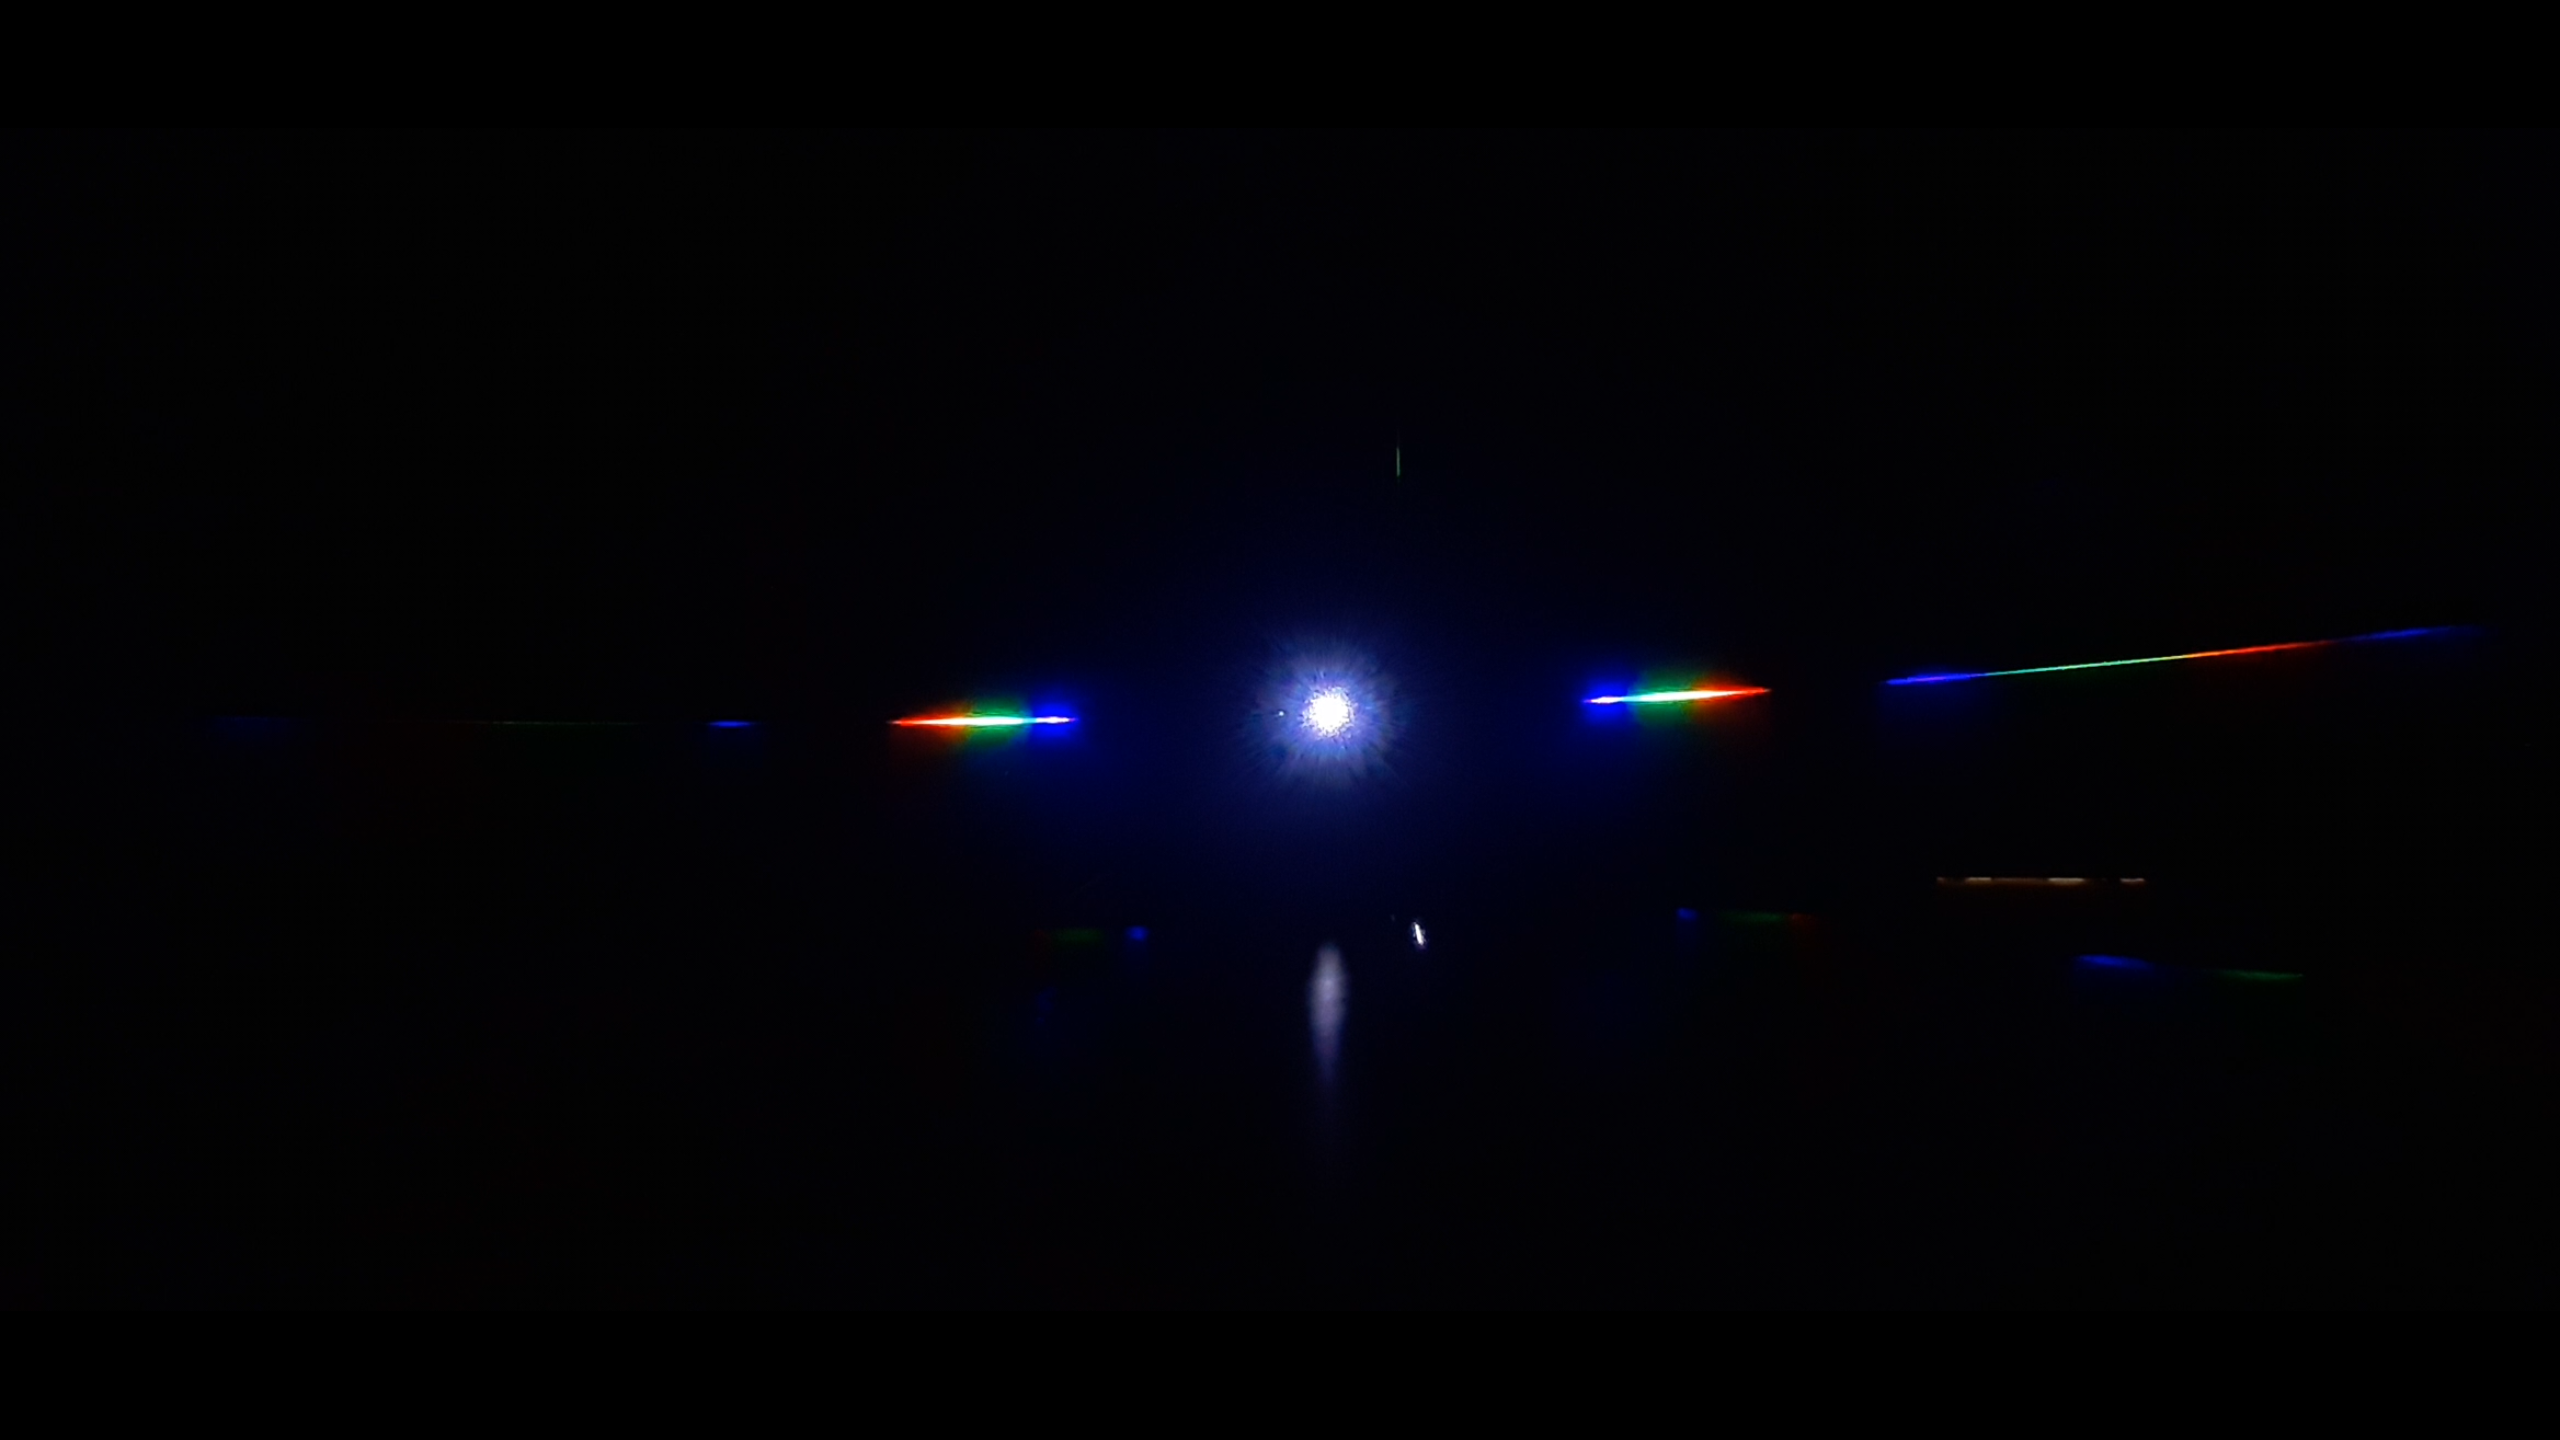
\includegraphics[scale=0.14]{Risultati Sperimentali/Primo reticoloT1.png} 
  \centering
  \qquad 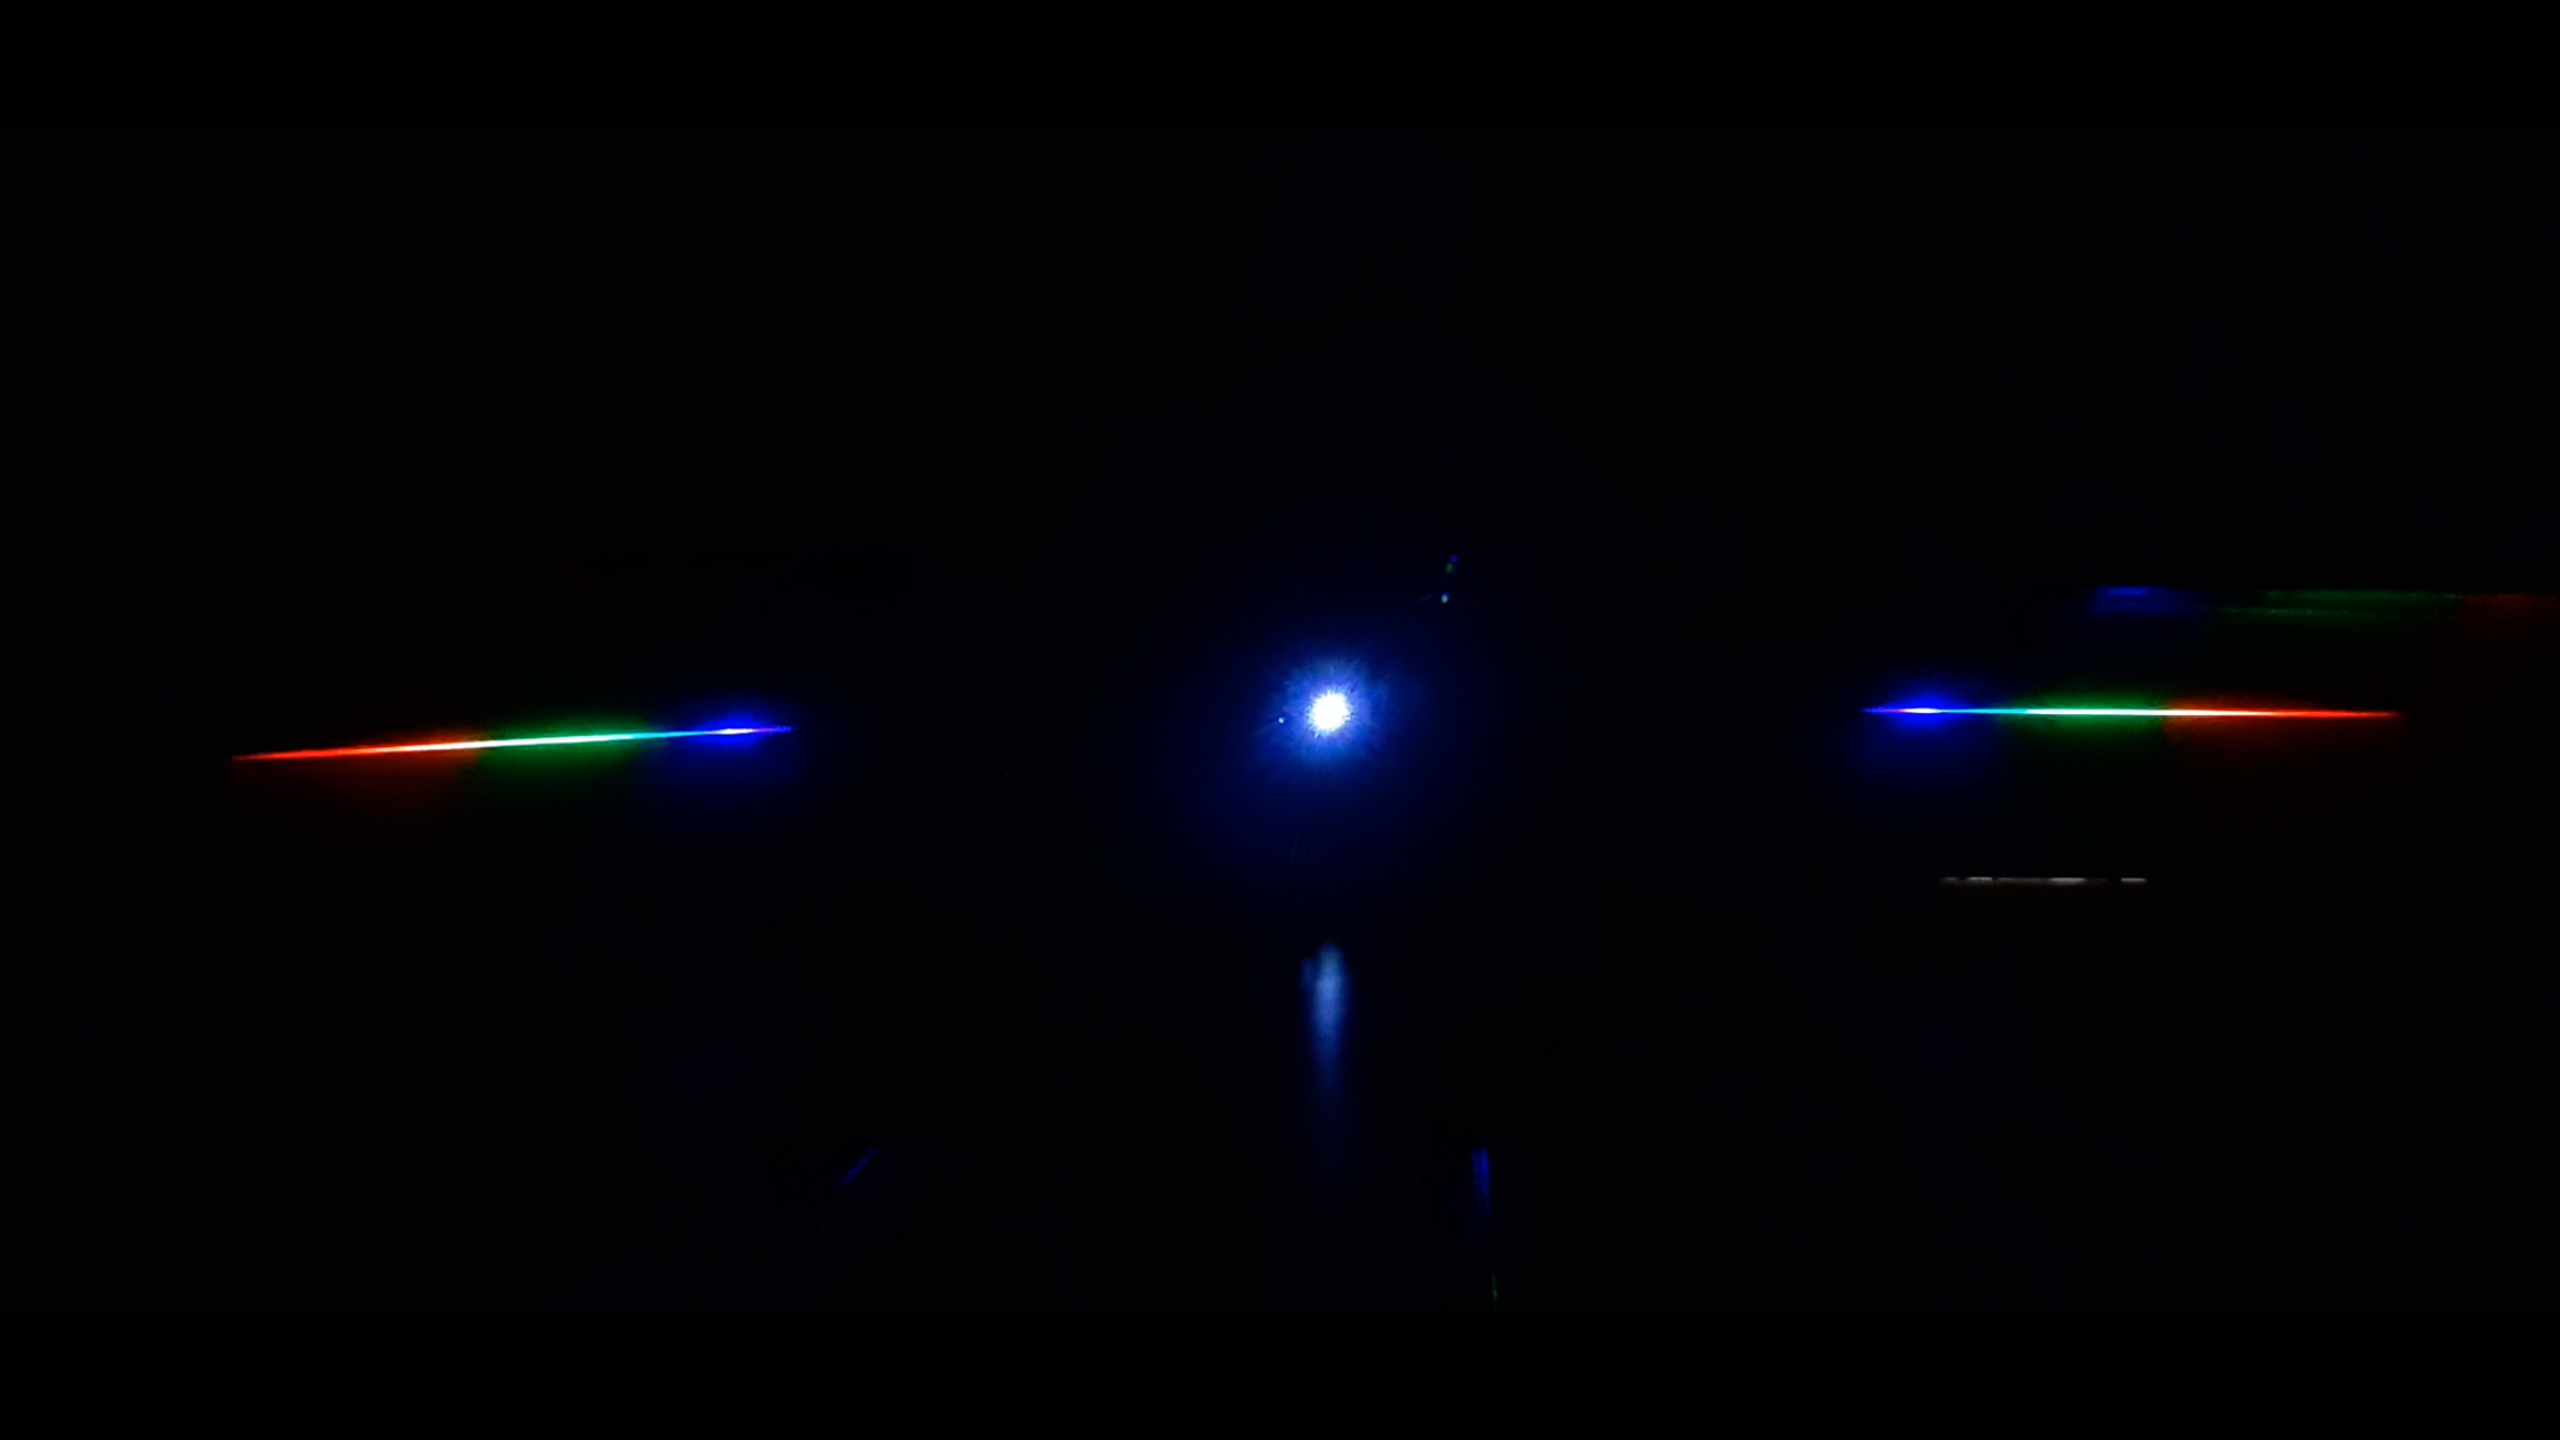
\includegraphics[scale=0.14]{Risultati Sperimentali/Secondo reticoloT1.png}
  \caption{In the first image it is possible to visualize the diffraction produced by the first holographic grating (with $d$ known) and in the second that produced by the second holographic grating (with $d'$ unknown). }
\end{figure}
\newpage
Obtaining the following results:
\begin{table}[ht!]
    \begin{tabular}{|c|c|c|c|c|c|}
    \hline
     $z\pm\sigma_z$ [mm] & $d$ [mm] & $\Delta x\pm\sigma_{\Delta x}$ [mm] & $\lambda\pm\sigma_\lambda$ [nm] & $\Delta x' \pm \sigma_{\Delta x'}$ [mm] & $d'\pm\sigma_{d'}$ [mm] \\
    \hline
    $4223\pm10$ & $0.002$ & $1093\pm15$ & $517.88\pm7.21$ & $2322\pm15$ & $(9.42\pm0.14)\times10^{-4}$ \\
    \hline
    \end{tabular}
    \caption{This table shows all the values with relative uncertainties measured and calculated during the first experience.}
\end{table}


The uncertainty related to $ d '$ was calculated through error propagation:
\begin{equation}
    \sigma_{d'}=\sqrt{\left(\frac{\lambda}{\Delta x}\right)^2\sigma_z^2+\left(\frac{\lambda z}{\Delta x'^2}\right)^2\sigma_{\Delta x'}^2+\left(\frac{z}{\Delta x}\right)^2\sigma_\lambda^2}
    \label{incertezza}
\end{equation}
Regarding the uncertainty $ \sigma_\lambda $ was obtained in a similar way using error propagation:
\begin{equation}
    \sigma_\lambda=\frac{\Delta x d}{z}
\end{equation}
For the uncertainty related to the measures of $ \Delta x $, $ \Delta x '$ and $ z $ they were chosen in a arbitrary way as it was difficult for me to quantify and calculate the error associated with these measures. For this reason I preferred to risk overestimating the error associated with direct measurements.
Ultimately getting $\text{liness/mm}=N$:
\begin{equation*}
    N=\frac{1}{d'}=(1061\pm17) \text{lines/mm}
\end{equation*}
I obtained the uncertainty related to lines/mm trhough error propagation:
\begin{equation}
    \sigma_N=\frac{1}{d'^2}\sigma_d'
\end{equation}
Using the second method without the wide-angle camera I obtained qualitatively consistent values:
\begin{table}[ht!]
    \begin{tabular}{|c|c|c|c|c|c|}
    \hline
     $z\pm\sigma_z$ [mm] & $d$ [mm] & $\Delta x\pm\sigma_{\Delta x}$ [mm] & $\lambda\pm\sigma_\lambda$ [nm] & $\Delta x' \pm \sigma_{\Delta x'}$ [mm] & $d'\pm\sigma_{d'}$ [mm] \\
    \hline
    $4223\pm10$ & $0.002$ & $985\pm15$ & $466.86\pm7.19$ & $2090\pm15$ & $(9.42\pm0.14)\times10^{-4}$ \\
    \hline
    \end{tabular}
    \caption{This table shows all the values with relative uncertainties measured and calculated during the first experience.}
\end{table}

From this I deduced that the wide angle does not modify the measurements taken in any way, you can view the images in the appendix.
\newpage
\subsection{First Bulb}
For the two bulbs I decided to change the measurement method: instead of making a continuous video and extracting the frames I decided to take single photos in the different configurations. These are the best images obtained by studying the first light bulb:
\begin{figure}[htp!]
  \centering
  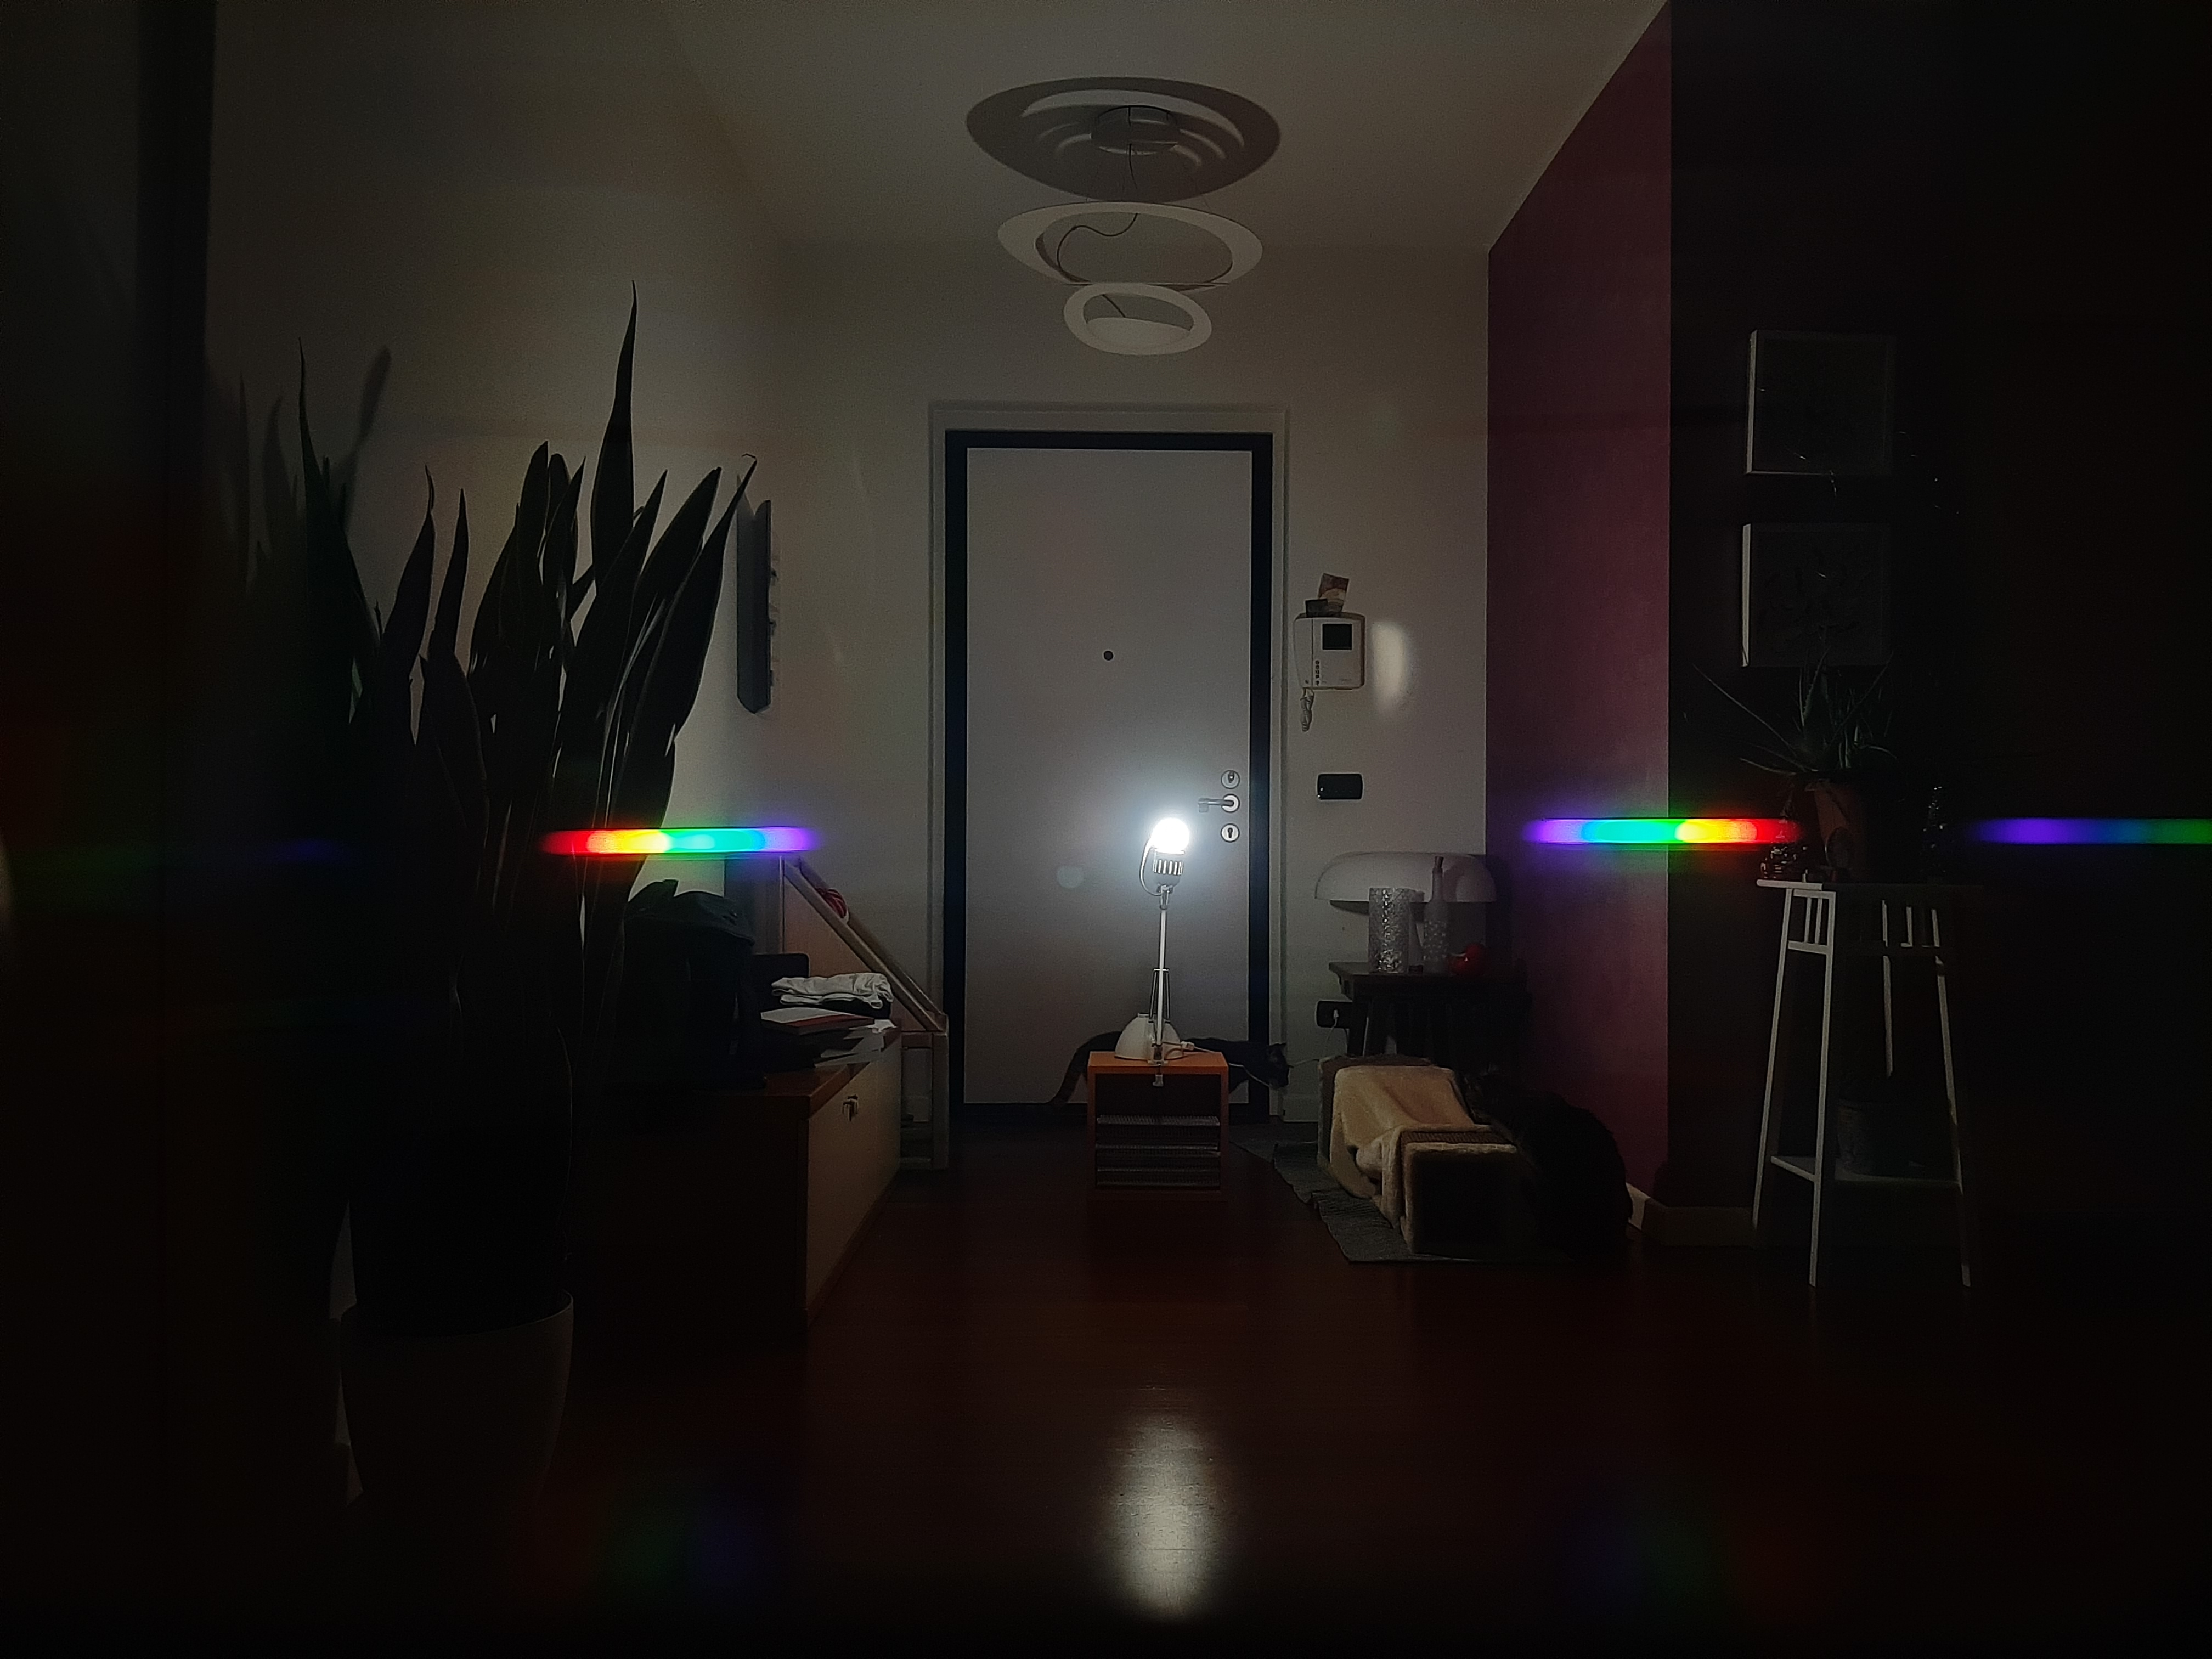
\includegraphics[scale=0.08]{Risultati Sperimentali/Lampada1a.jpg} 
  \centering
  \qquad 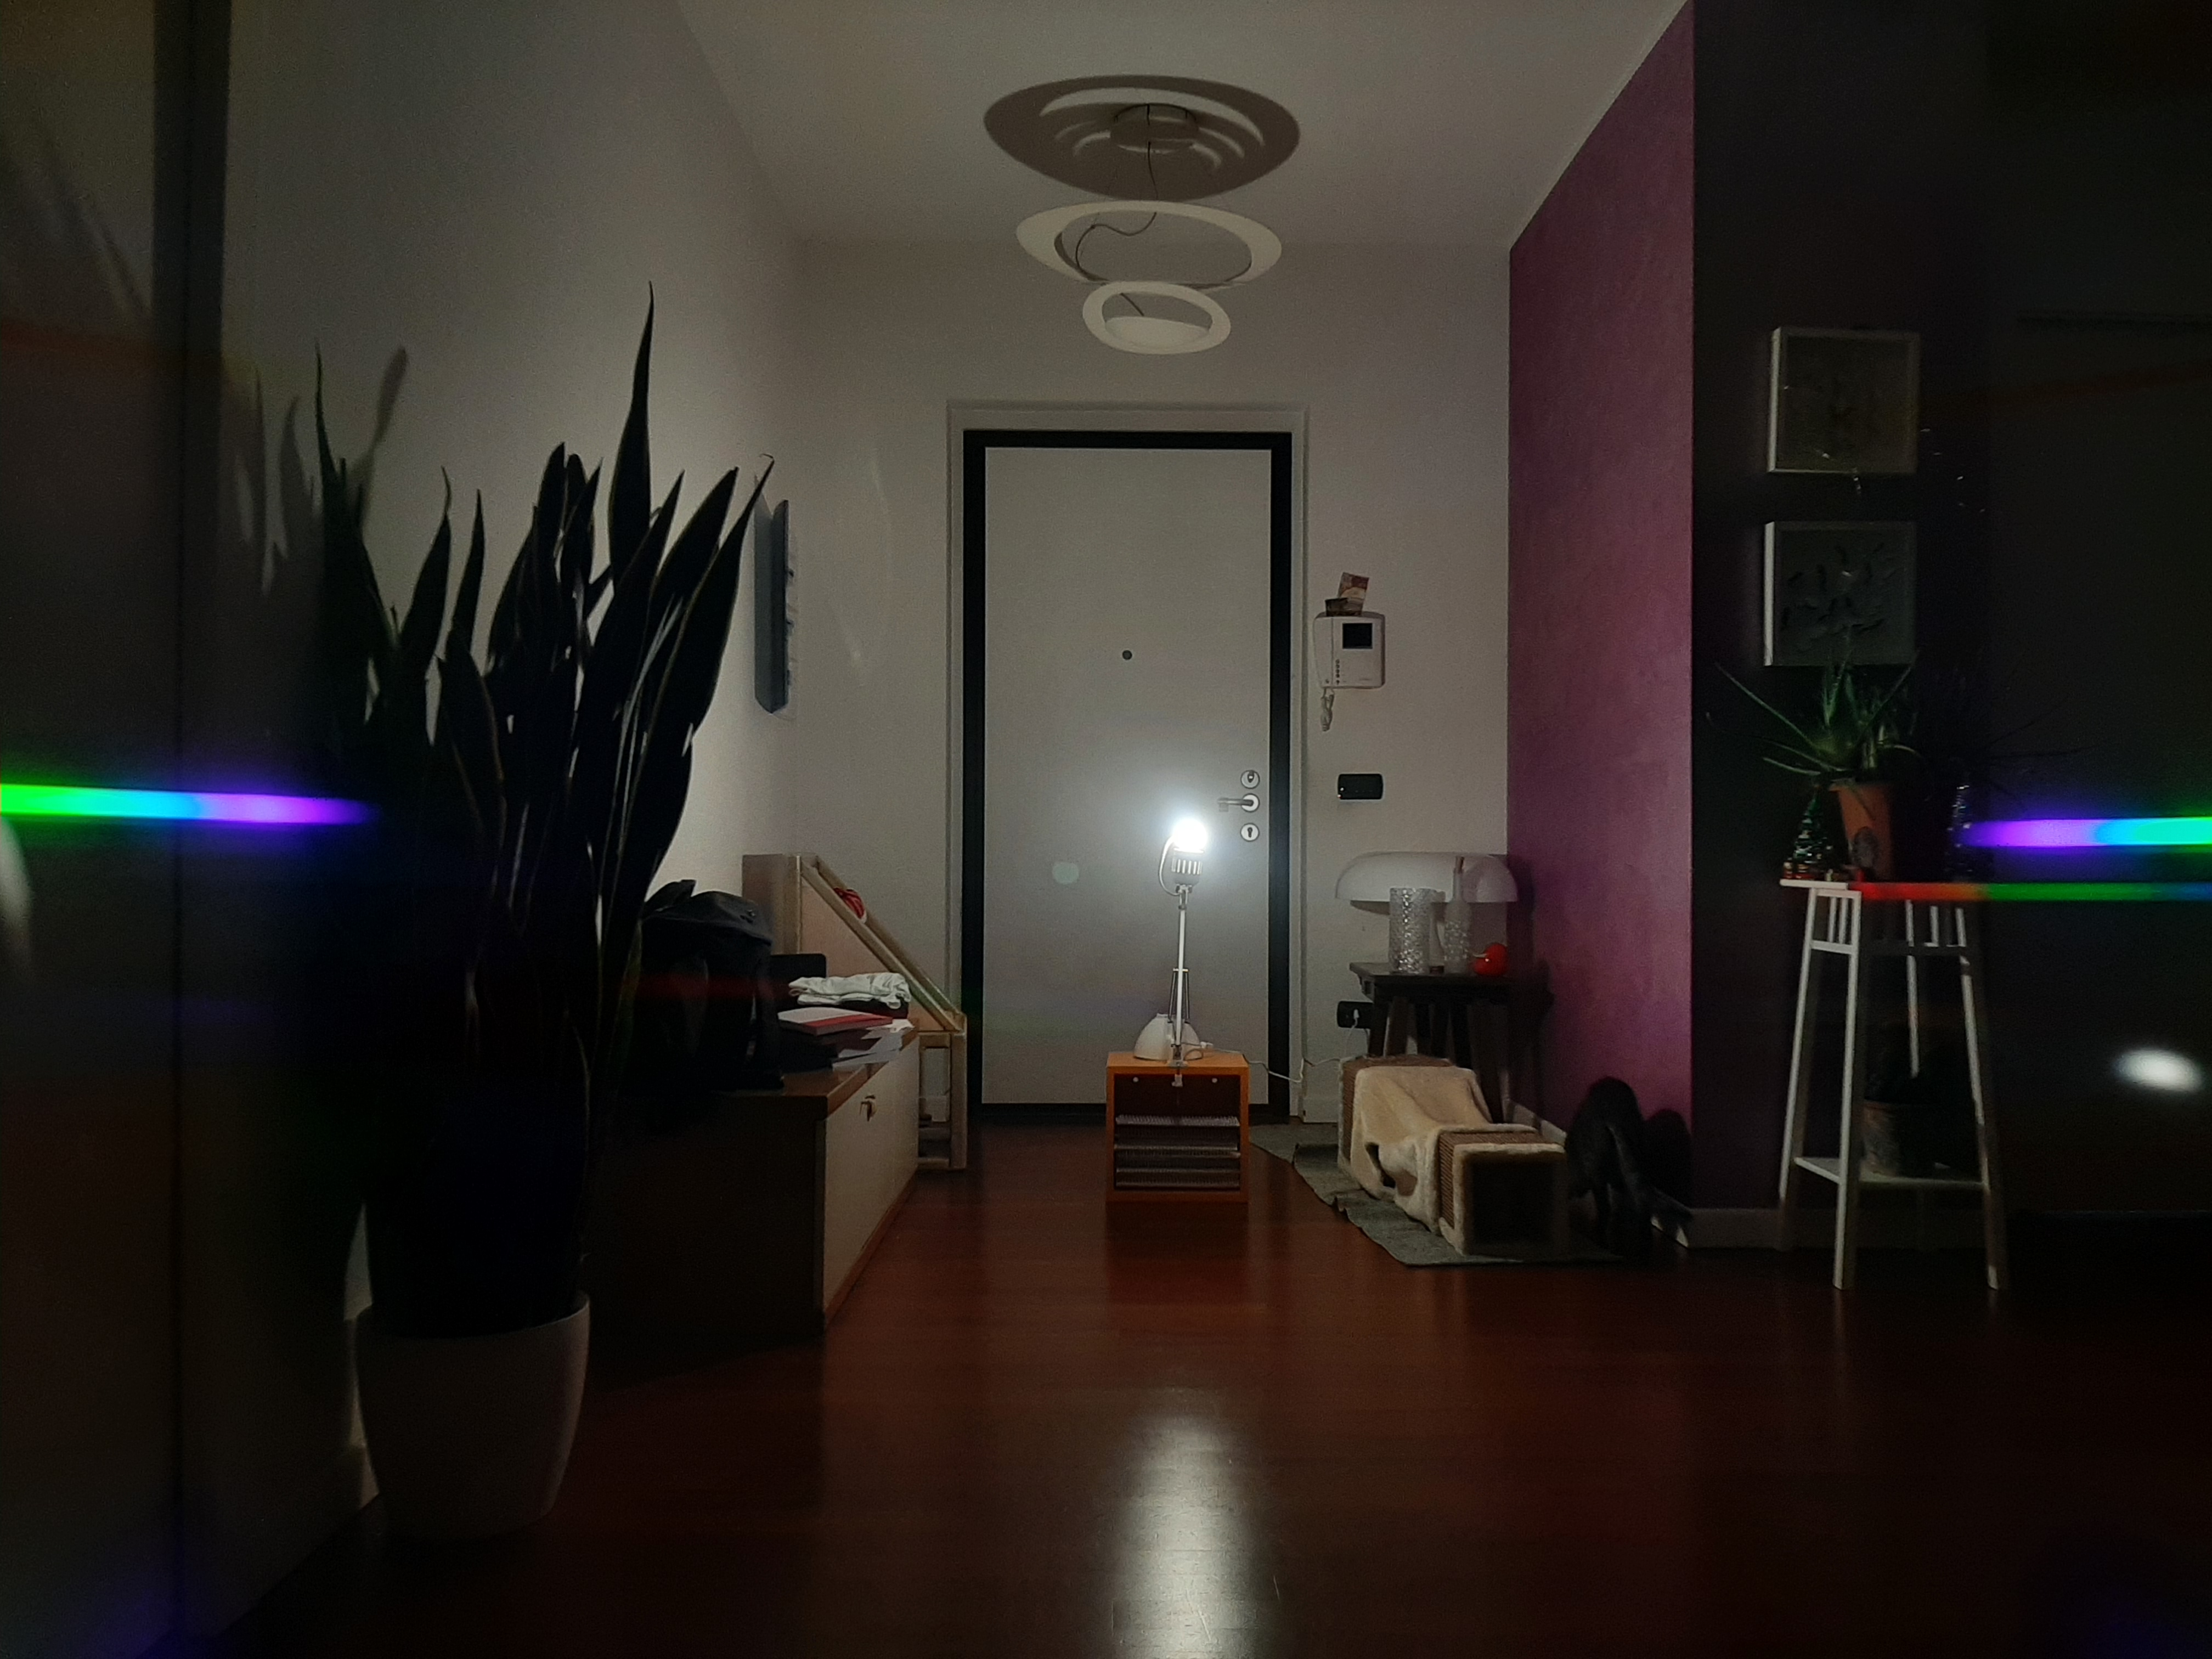
\includegraphics[scale=0.08]{Risultati Sperimentali/Lampada1b.jpg}
  \caption{In the first image it is possible to visualize the diffraction produced by the first holographic grating (with $d$ known) and in the second that produced by the second holographic grating (with $d'$ unknown). }
\end{figure}


Obtaining the following results shown in the table (\ref{t}).
\begin{table}[ht!]
    \begin{tabular}{|c|c|c|c|c|c|}
    \hline
     $z\pm\sigma_z$ [mm] & $d$ [mm] & $\Delta x\pm\sigma_{\Delta x}$ [mm] & $\lambda\pm\sigma_\lambda$ [nm] & $\Delta x' \pm \sigma_{\Delta x'}$ [mm] & $d'\pm\sigma_{d'}$ [mm] \\
    \hline
    $3730\pm10$ & $0.002$ & $1003\pm15$ & $538.05\pm8.17$ & $2180\pm15$ & $(9.20\pm0.16)\times10^{-4}$ \\
    \hline
    \end{tabular}
    \caption{This table shows all the values with relative uncertainties measured and calculated during the first experience.}
    \label{t}
\end{table}
The uncertainty relative to the value $d'$ is obtained through the equation (\ref{incertezza}) and therefore I obtained:
\begin{equation*}
    N=\frac{1}{d'}=(1086\pm18) \text{lines/mm}
\end{equation*}
\subsection{Second bulb}
These are the images I got by studying the second bulb (warm light):
\begin{figure}[htp!]
  \centering
  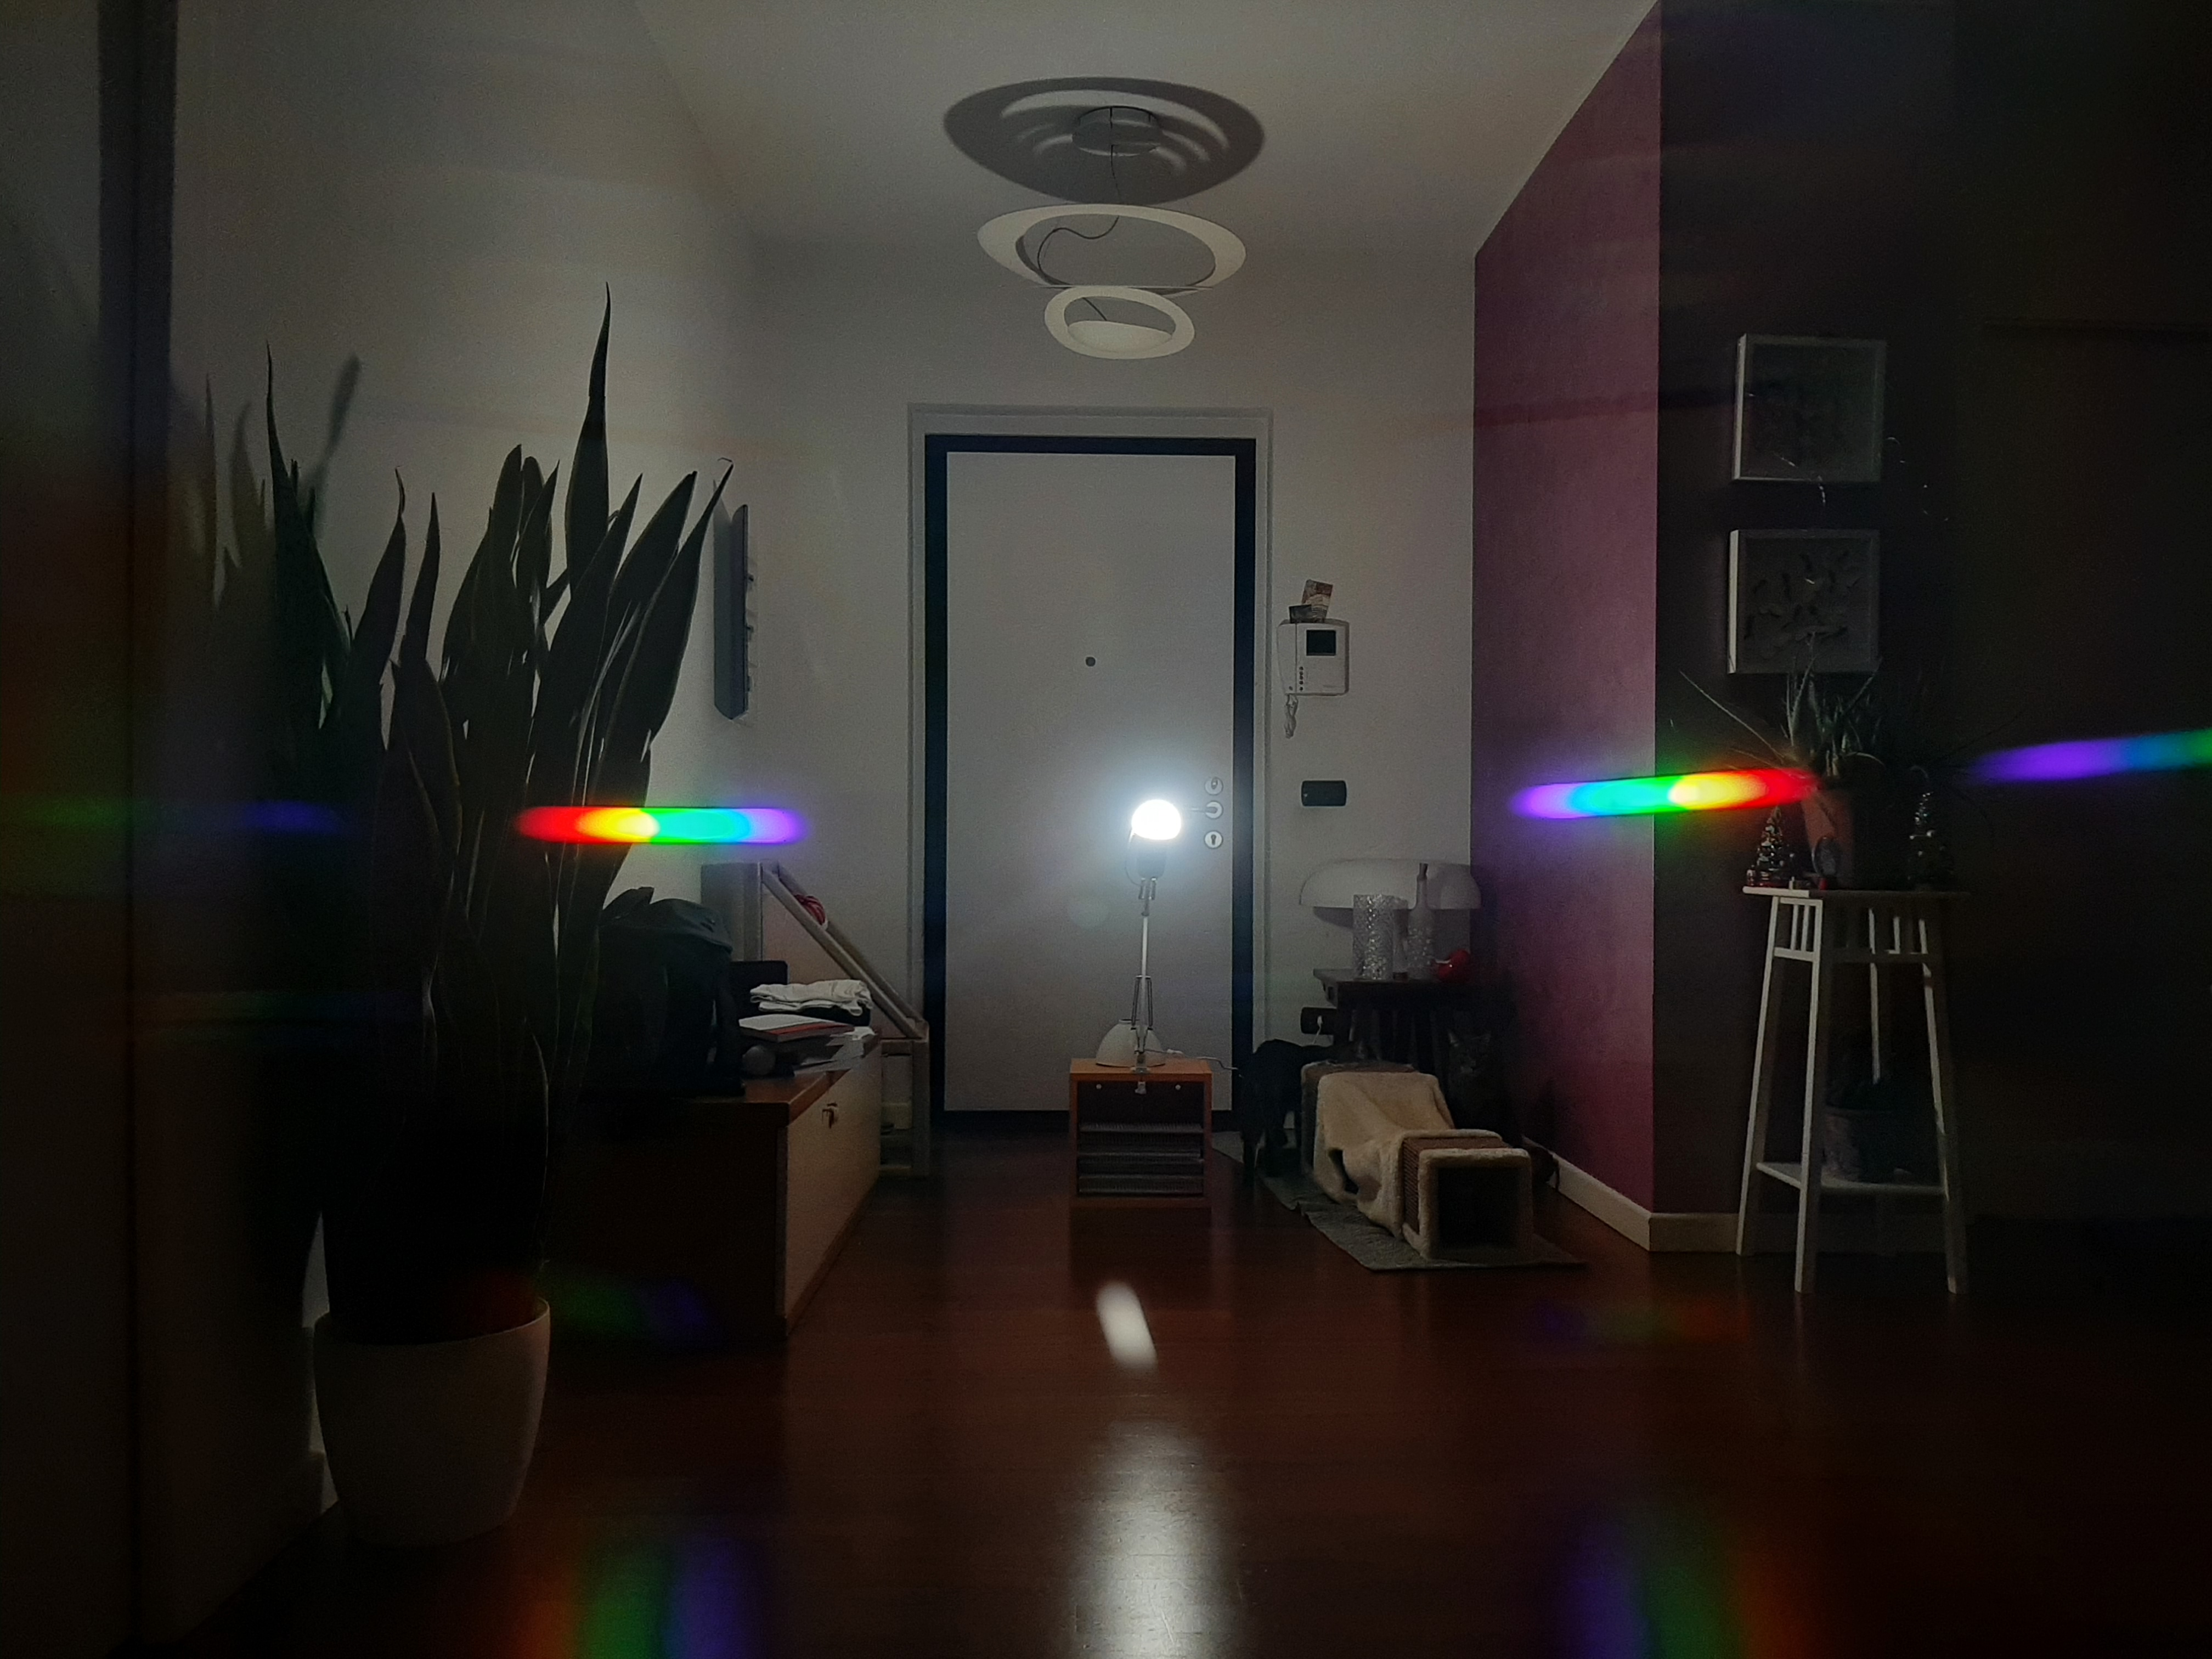
\includegraphics[scale=0.08]{Risultati Sperimentali/Lampada2a.jpg} 
  \centering
  \qquad 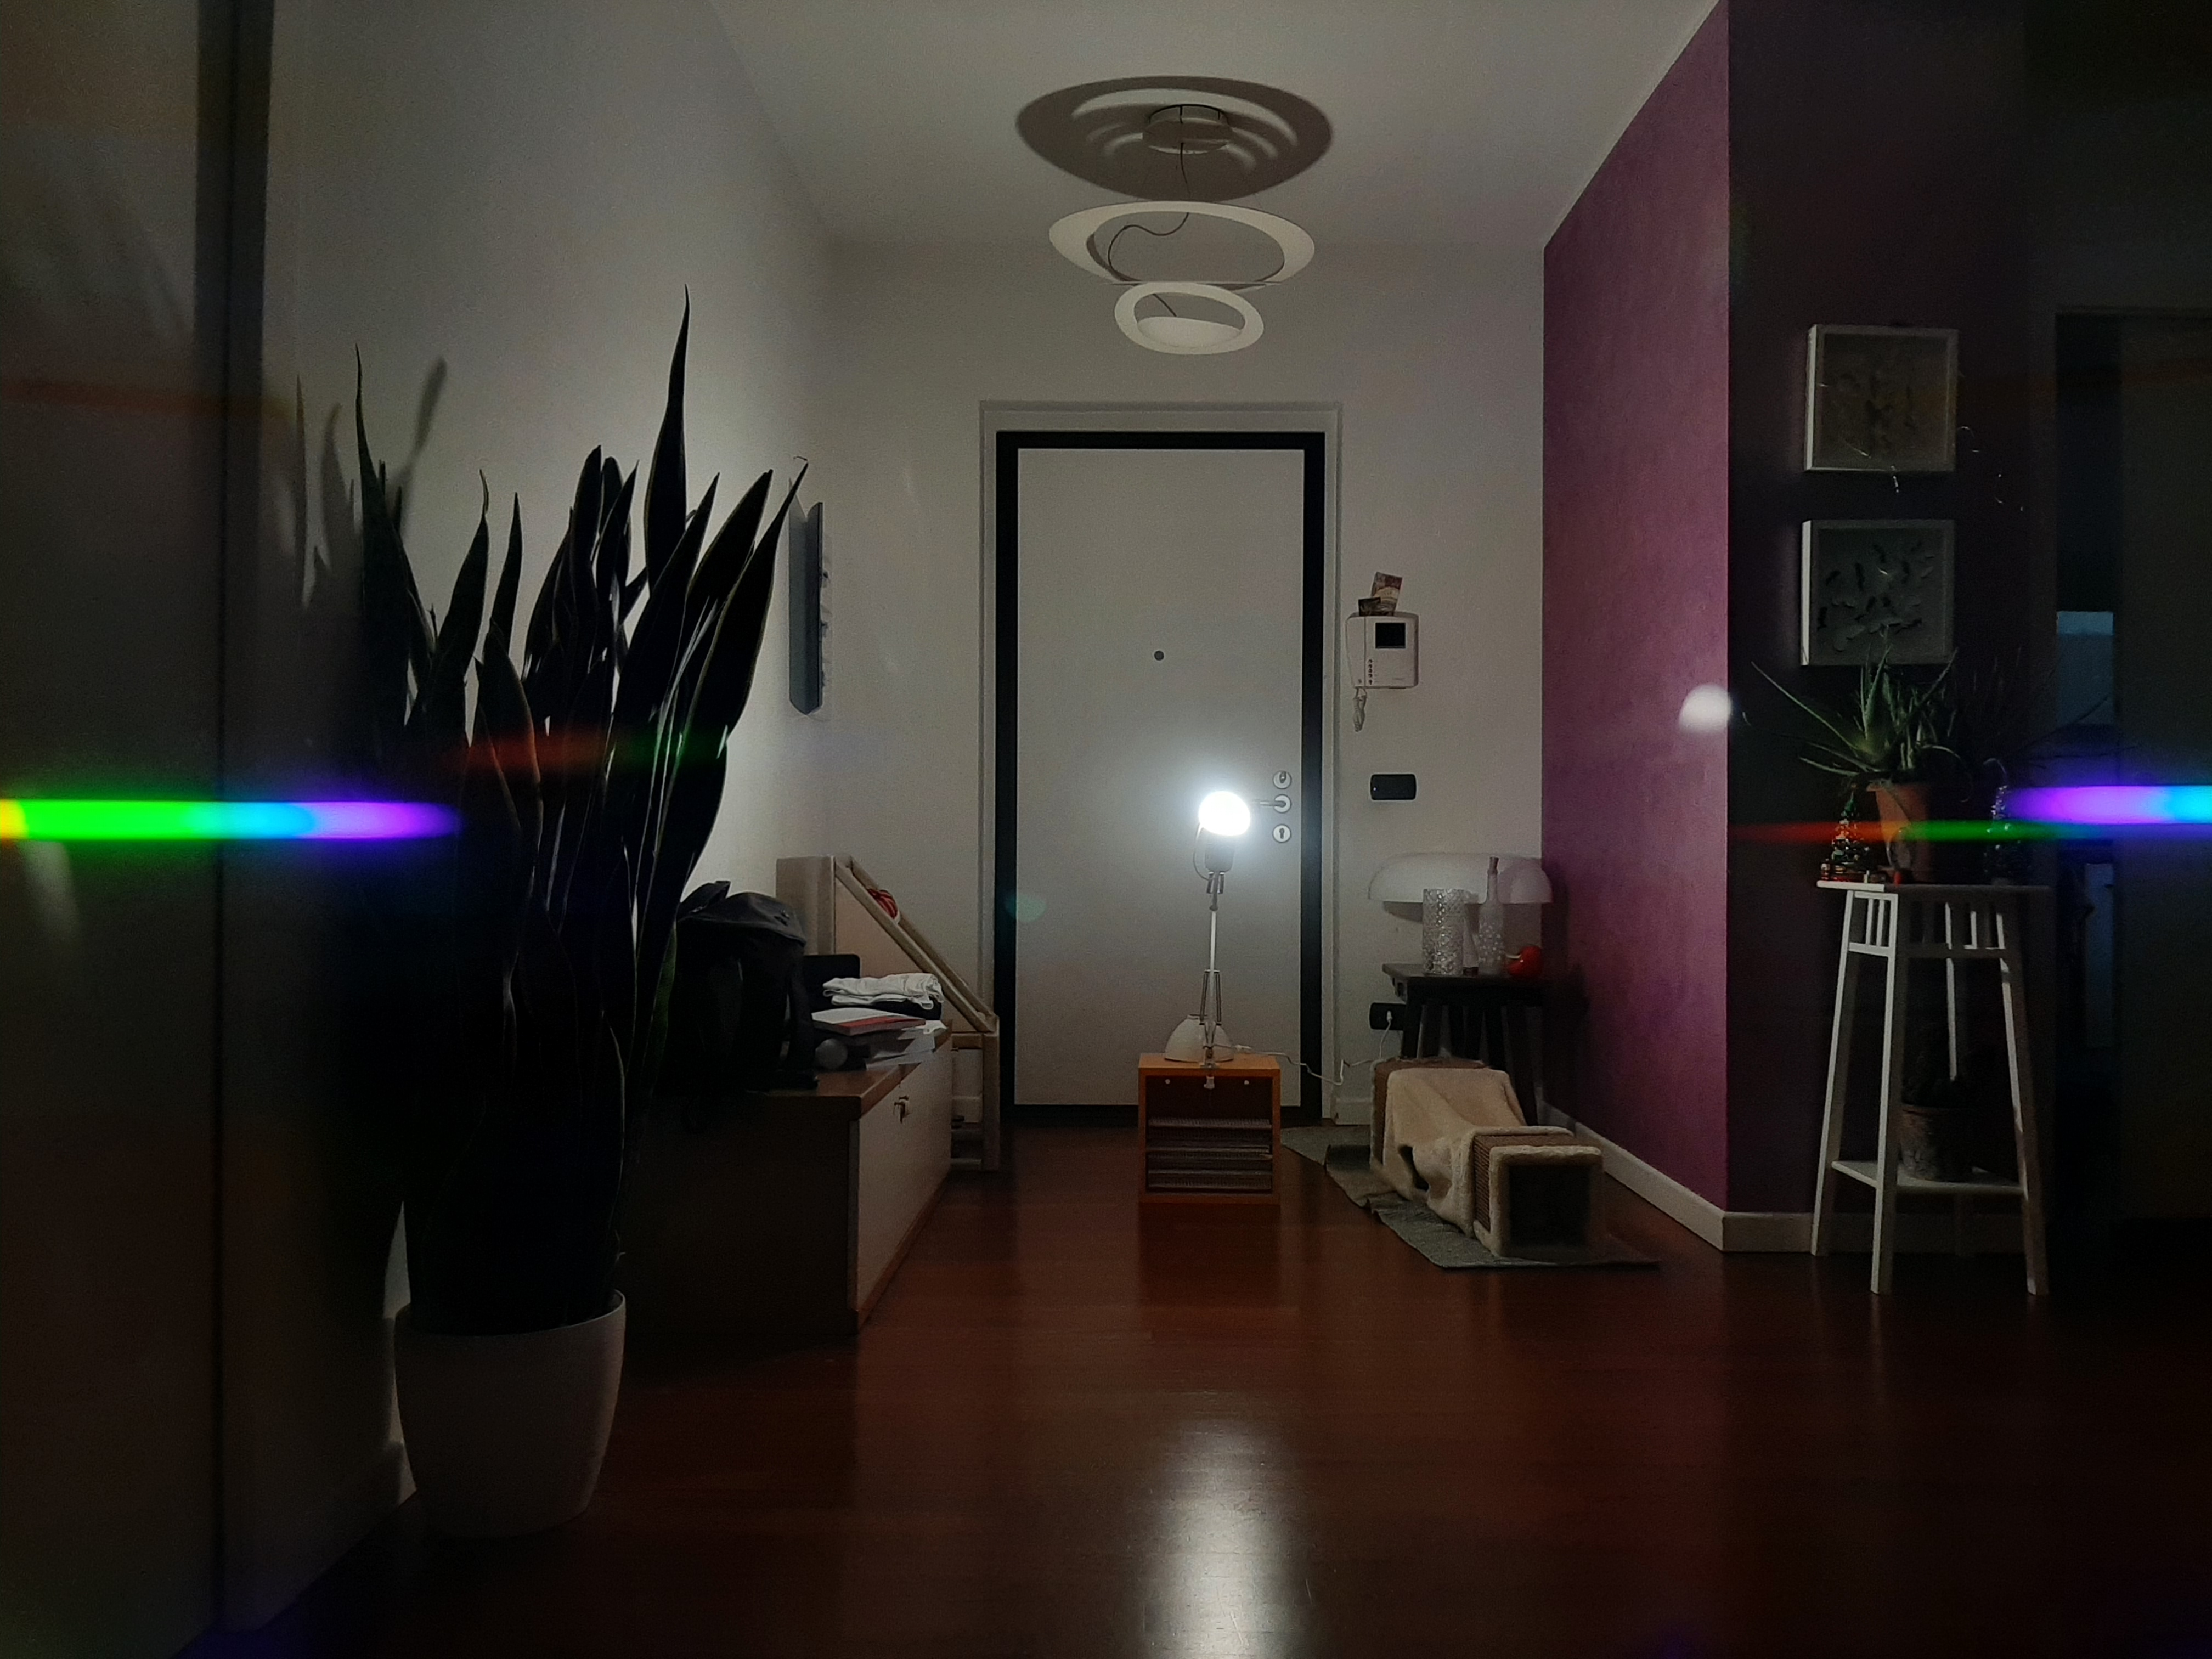
\includegraphics[scale=0.08]{Risultati Sperimentali/Lampada2b.jpg}
  \caption{In the first image it is possible to visualize the diffraction produced by the first holographic grating (with $d$ known) and in the second that produced by the second holographic grating (with $d'$ unknown). }
\end{figure}
\newpage
Obtaining the following results:
\begin{table}[ht!]
    \begin{tabular}{|c|c|c|c|c|c|}
    \hline
     $z\pm\sigma_z$ [mm] & $d$ [mm] & $\Delta x\pm\sigma_{\Delta x}$ [mm] & $\lambda\pm\sigma_\lambda$ [nm] & $\Delta x' \pm \sigma_{\Delta x'}$ [mm] & $d'\pm\sigma_{d'}$ [mm] \\
    \hline
    $3730\pm10$ & $0.002$ & $993\pm15$ & $532.97\pm8.17$ & $2126\pm15$ & $(9.34\pm0.16)\times10^{-4}$ \\
    \hline
    \end{tabular}
    \caption{This table shows all the values with relative uncertainties measured and calculated during the first experience.}
\end{table}


The uncertainty relative to the value $d'$ is obtained through the equation (\ref{incertezza}) and therefore I obtained:
\begin{equation*}
    N=\frac{1}{d'}=(1069\pm18) \text{lines/mm}
\end{equation*}

\section{Conclusion}
The objective of the experiment is to measure the $d'$ of a holographic grating using a second holographic grating with a known $d$. To do this I decided to study three different sources and try to use different methods. The values obtained are qualitatively consistent with each other even if they come from different configurations. During the data taking process I encountered some problems in quantifying the errors associated with direct measurements. In view of this, the goal has been achieved.
\newpage
\appendix
\section{Images taken without wide-angle}
\begin{figure}[htp!]
  \centering
  
\includegraphics[scale=0.07]{Conclusione/gg.png} 
  \centering
  \qquad 
\includegraphics[scale=0.07]{Conclusione/ff.png}
  \caption{These two images have been taken without wide angle.}
\end{figure}
\section{Measurement Methods}
Here are some images taken during the measurement of $ \Delta x $ using the Imagej software:
\begin{figure}[htp!]
  \centering
  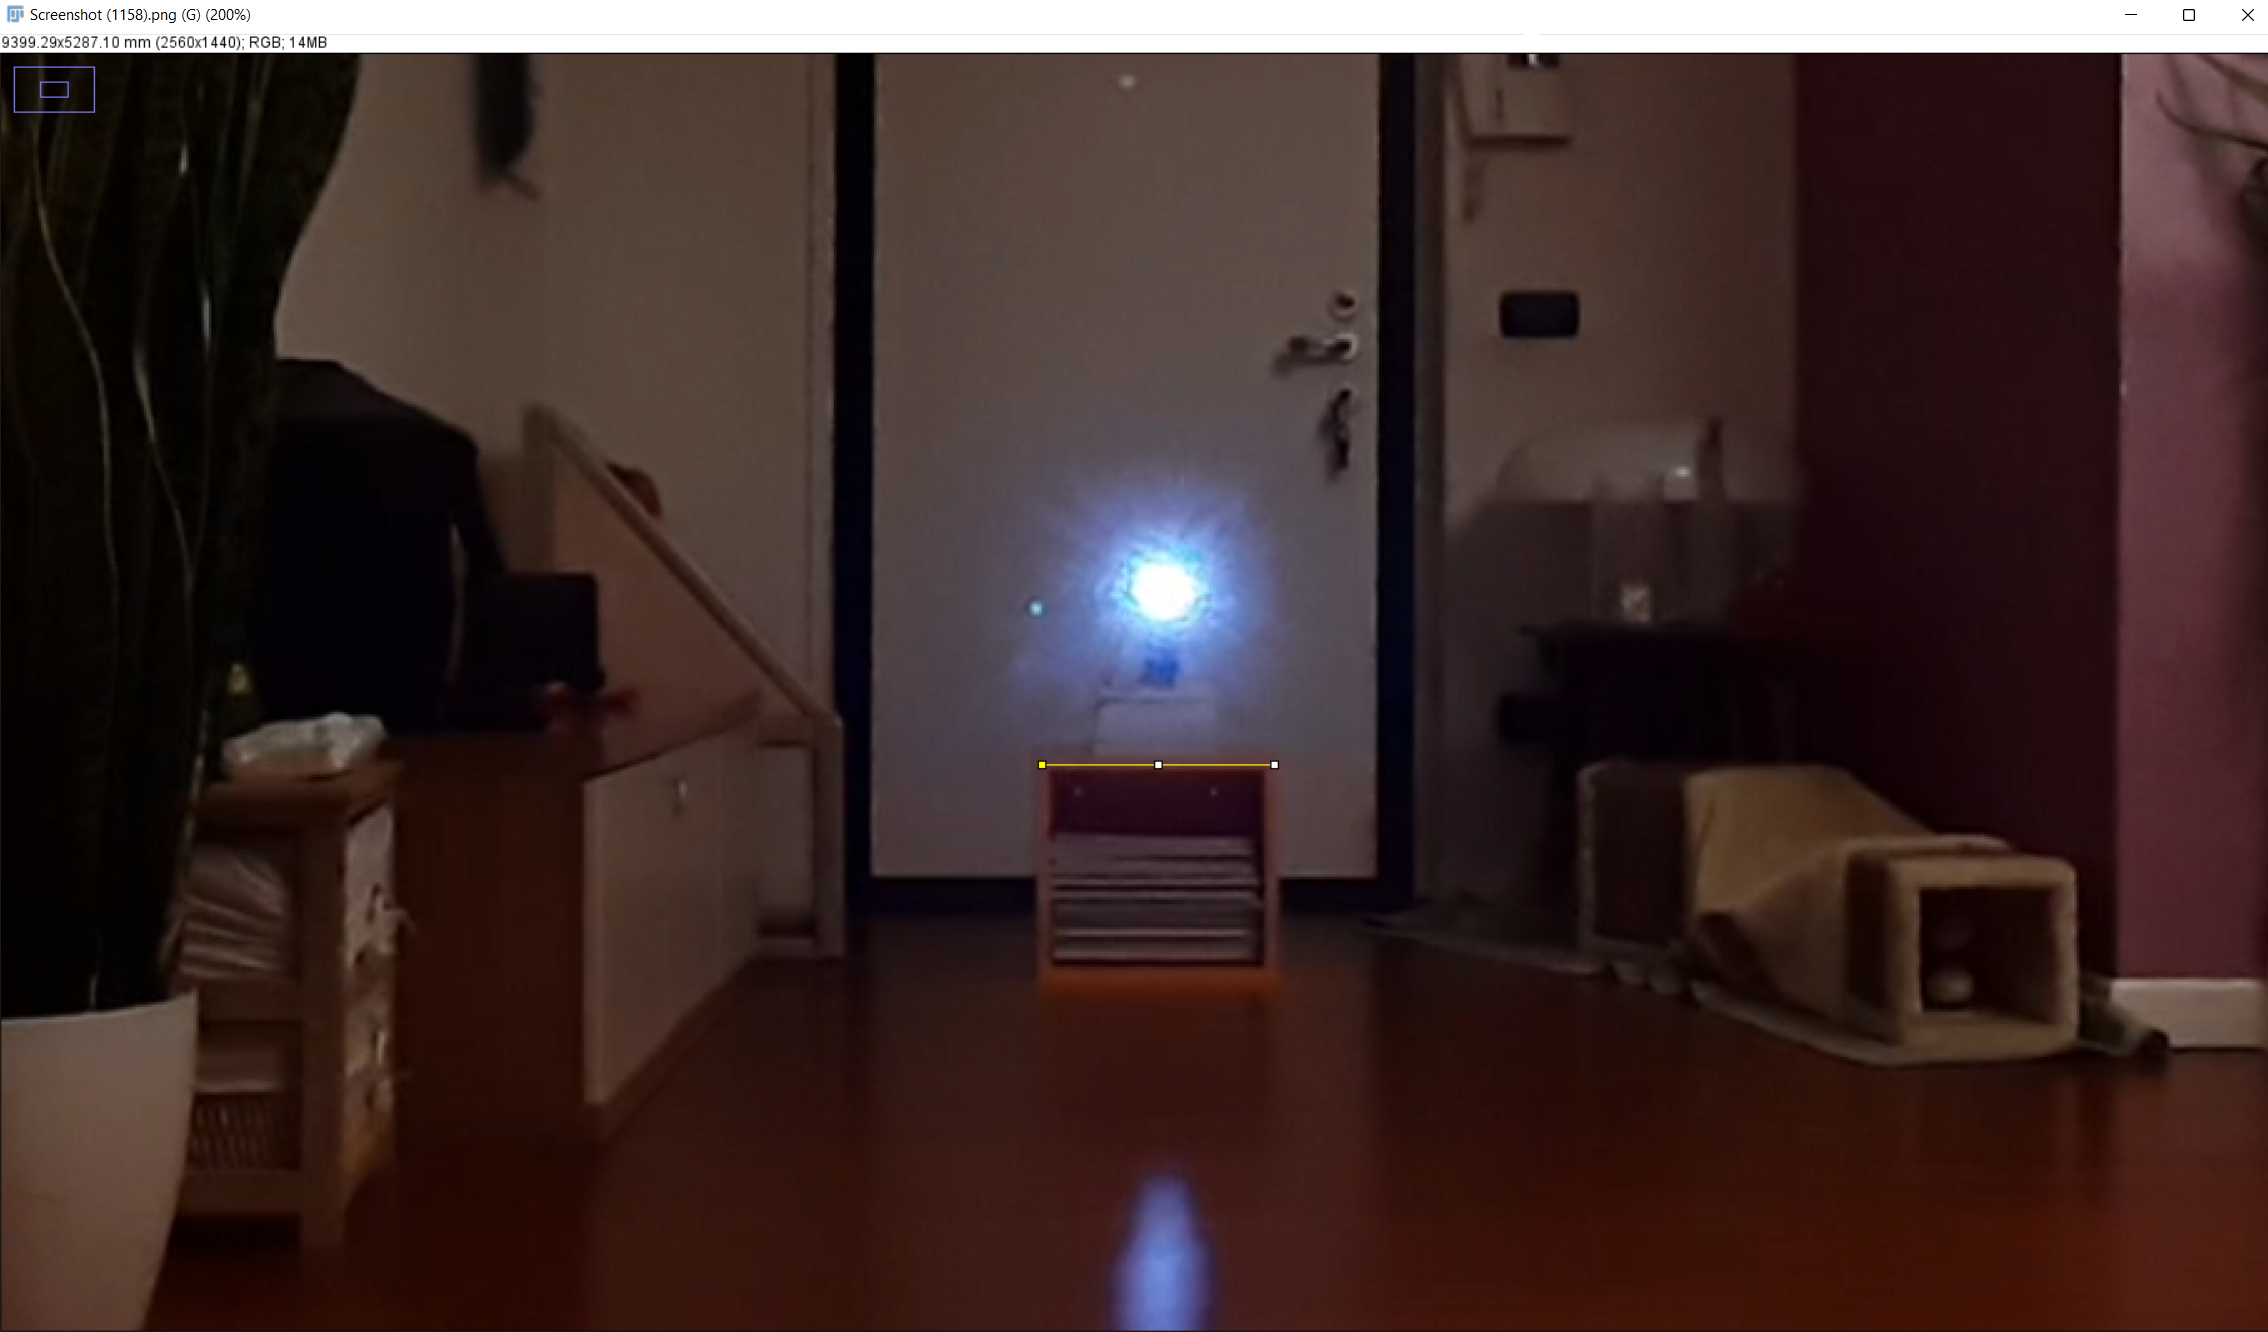
\includegraphics[scale=0.15]{Conclusione/Sist.png} 
  \centering
  \qquad 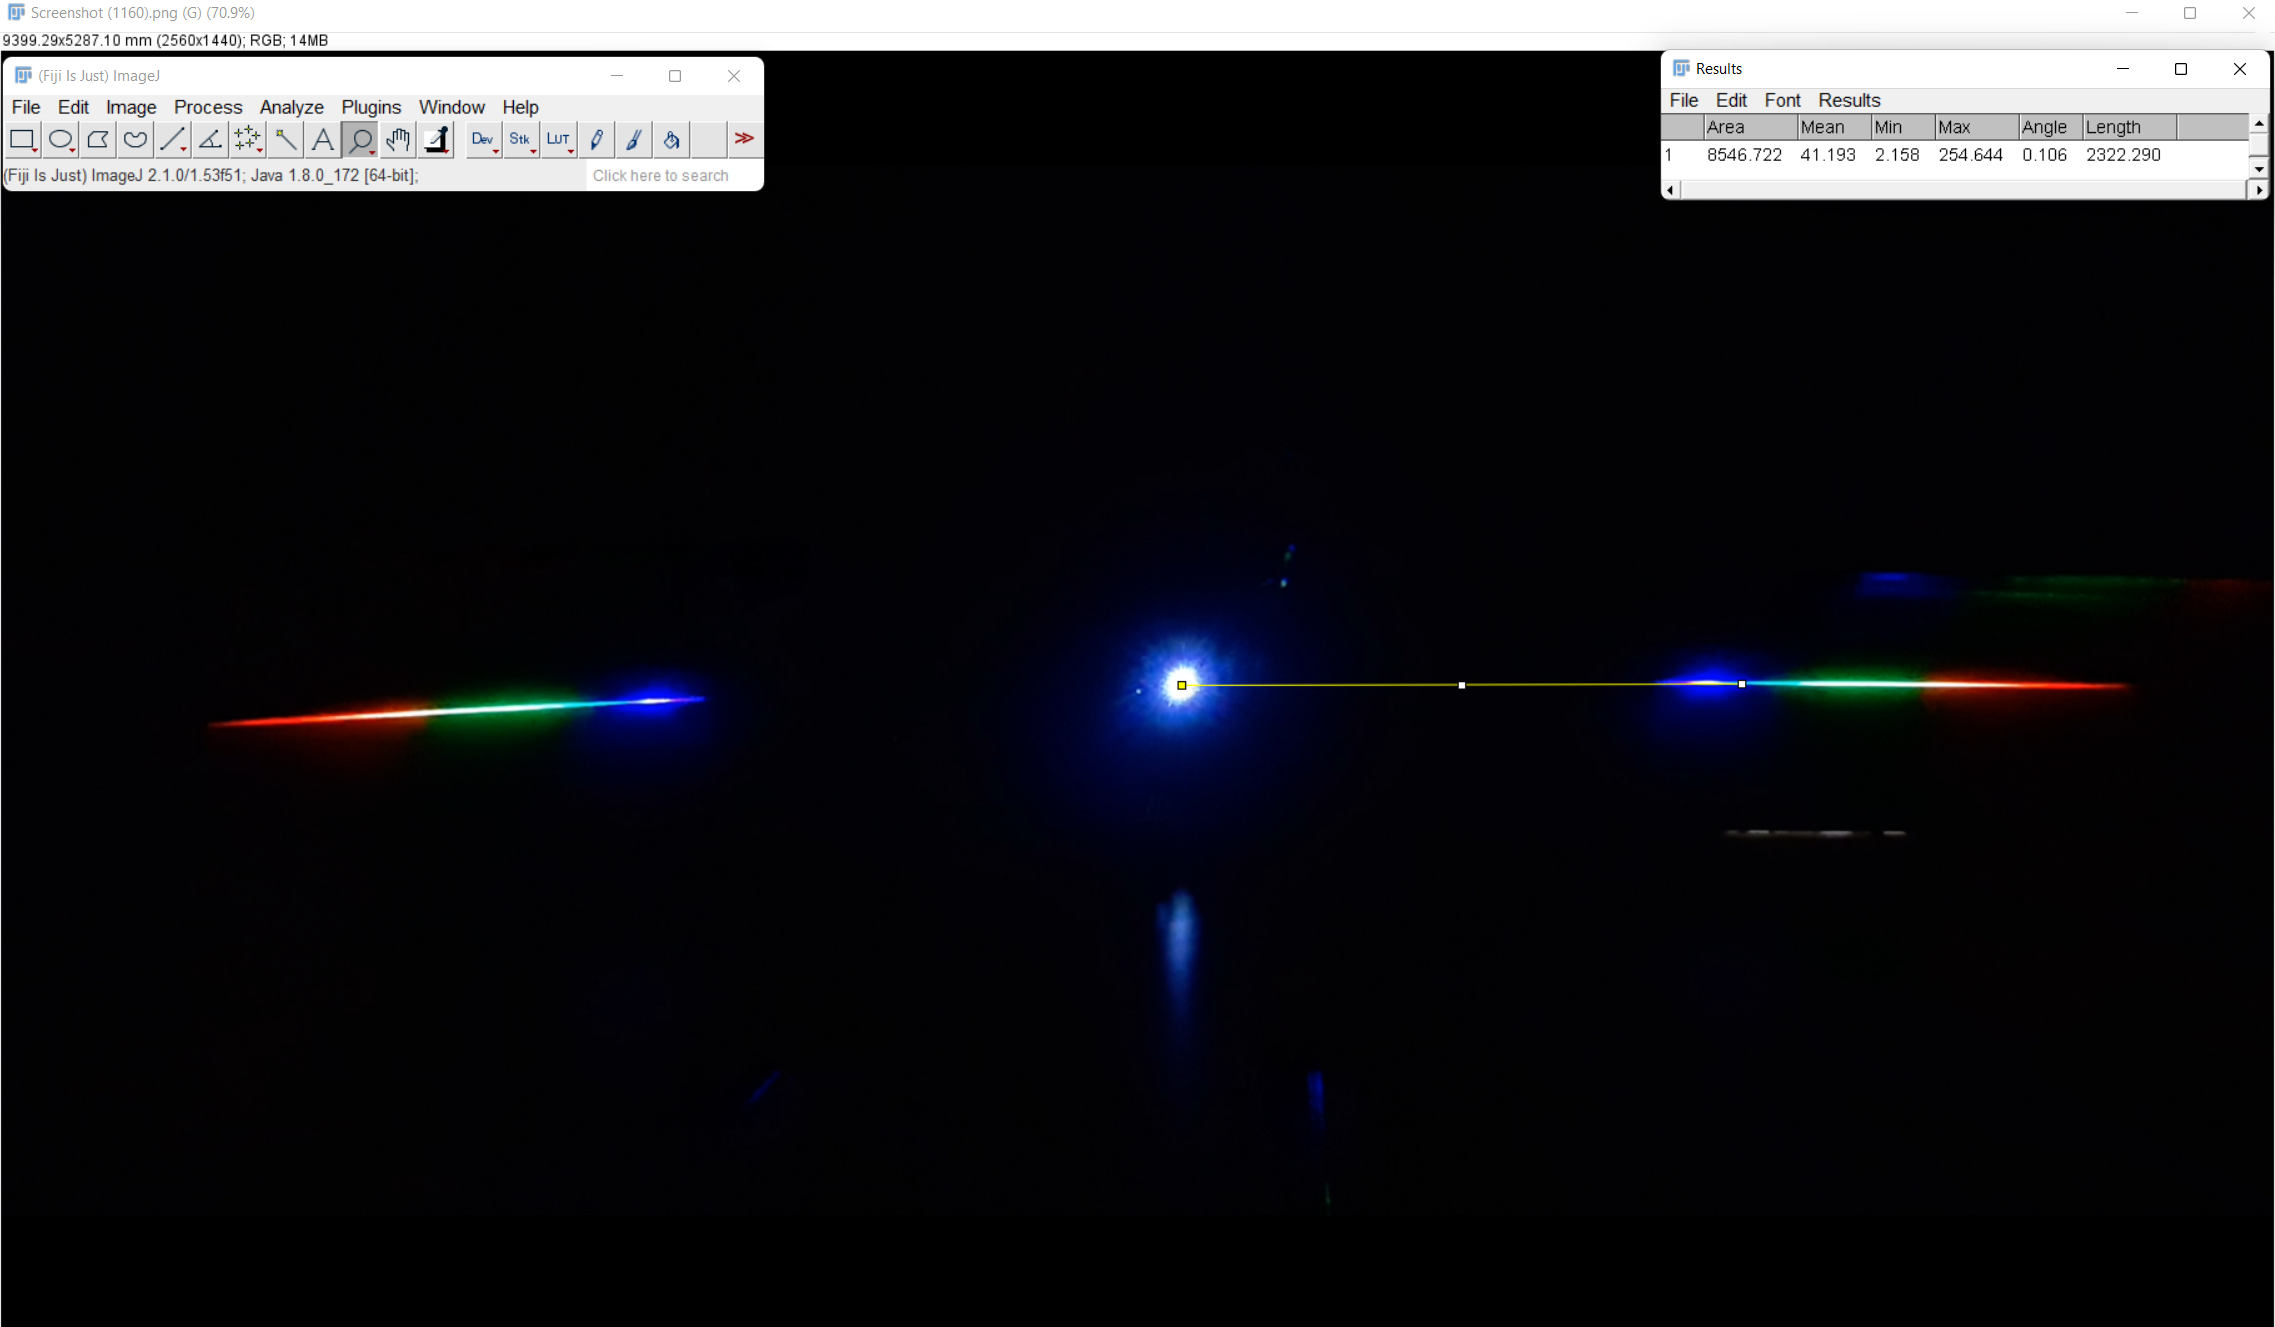
\includegraphics[scale=0.15]{Conclusione/mis.png}
  \caption{In these two images it is possible to visualize the way in which the distances between the real source and the virtual source have been measured.}
\end{figure}
\end{document}
